\documentclass[12pt]{article}
\usepackage[utf8]{inputenc}
\usepackage{float}
\usepackage{amsmath}
\usepackage[tableaux]{prooftrees}
\renewcommand*\linenumberstyle[1]{(#1)}

\usepackage[hmargin=3cm,vmargin=6.0cm]{geometry}
\topmargin=-2cm
\addtolength{\textheight}{6.5cm}
\addtolength{\textwidth}{2.0cm}
\setlength{\oddsidemargin}{0.0cm}
\setlength{\evensidemargin}{0.0cm}
\usepackage{indentfirst}
\usepackage{amsfonts}
\usepackage{tikz}
\usepackage{qtree}
% \usepackage{pmatrix}

\begin{document}

\section*{Student Information}

Name: Kaan Karaçanta \\

ID: 2448546 \\


\section*{Part 1}

\subsection*{\text{a)}}

To show whether the gate \( U_f \) is invertible or not, we consider the properties of quantum gates. A gate \( U_f \) acts on two qubits as follows:

\[
U_f |x\rangle |y\rangle = |x\rangle |y \oplus f(x)\rangle
\]

where \( \oplus \) denotes addition modulo 2 (XOR operation). For \( U_f \) to be invertible, there must exist a \( U_f^{-1} \) such that:

\[
U_f^{-1}U_f |x\rangle |y\rangle = |x\rangle |y\rangle
\]

Since \( a \oplus b \oplus b = a \) for binary variables \( a \) and \( b \), applying \( U_f \) twice will return the original state:

\[
U_f U_f |x\rangle |y\rangle = U_f |x\rangle |y \oplus f(x)\rangle = |x\rangle |y \oplus f(x) \oplus f(x)\rangle = |x\rangle |y\rangle
\]

Thus, \( U_f \) is invertible.

\subsection*{\text{b)}}

To compute the result of \( U_f (H \otimes I) (|0\rangle \otimes |1\rangle) \) for \( f(x) = \neg x \), apply each gate in sequence:

First, apply the Hadamard gate \( H \) to \( |0\rangle \) and the identity \( I \) to \( |1\rangle \):

\[
(H \otimes I) (|0\rangle \otimes |1\rangle) = (H|0\rangle) \otimes (I|1\rangle)
\]

The Hadamard gate \( H \) transforms \( |0\rangle \) to a superposition:

\[
H|0\rangle = \frac{1}{\sqrt{2}}(|0\rangle + |1\rangle)
\]

Thus:

\[
(H \otimes I) (|0\rangle \otimes |1\rangle) = \frac{1}{\sqrt{2}}(|0\rangle + |1\rangle) \otimes |1\rangle = \frac{1}{\sqrt{2}}(|01\rangle + |11\rangle)
\]

Now apply \( U_f \) with \( f(x) = \neg x \):

\[
U_f |x\rangle |y\rangle = |x\rangle |y \oplus \neg x\rangle
\]

\newpage

For \( |01\rangle \):

\[
U_f |01\rangle = |0\rangle |1 \oplus \neg 0\rangle = |0\rangle |1 \oplus 1\rangle = |00\rangle
\]

For \( |11\rangle \):

\[
U_f |11\rangle = |1\rangle |1 \oplus \neg 1\rangle = |1\rangle |1 \oplus 0\rangle = |11\rangle
\]

The final state is:

\[
U_f \left(\frac{1}{\sqrt{2}}(|01\rangle + |11\rangle)\right) = \frac{1}{\sqrt{2}}(|00\rangle + |11\rangle)
\]

This is the result after applying \( U_f \) to the superposition created by \( H \) and \( I \).


% f(x) = x and f : {0, 1} → {0, 1}
\subsection*{\text{c)}}

This is a balanced function and here is the implementation of the circuit and measurement outcome:

\begin{figure}[H]
    \centering
    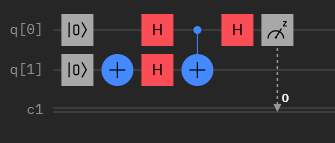
\includegraphics[scale=0.9]{1c.png}
    \caption{The circuit}
\end{figure}

\begin{figure}[H]
    \centering
    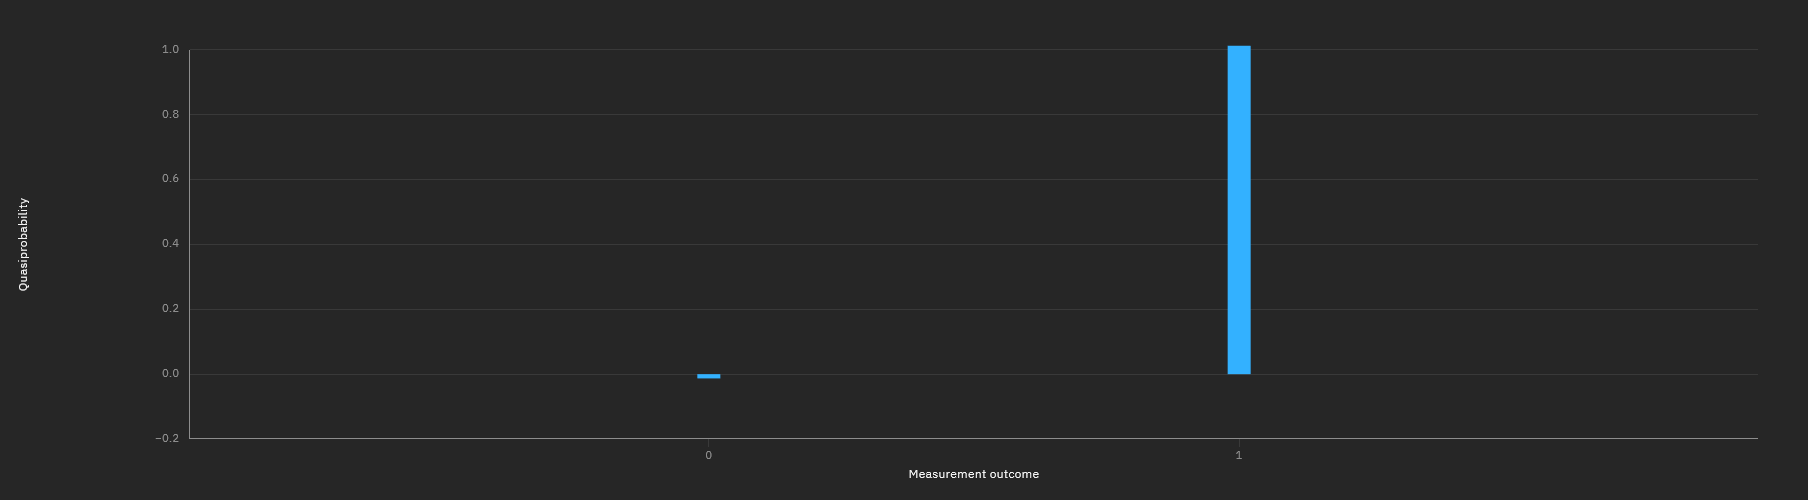
\includegraphics[scale=0.27]{1cr.png}
    \caption{The results of the measurement of the circuit after 1024 shots.}
\end{figure}

\newpage

% f(x) = 1 and f : {0, 1} → {0, 1}
\subsection*{\text{d)}}

This is a constant function and here is the implementation of the circuit and measurement outcome:

\begin{figure}[H]
    \centering
    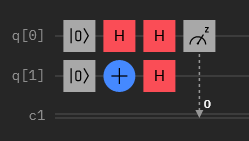
\includegraphics[scale=0.9]{1d.png}
    \caption{The circuit}
\end{figure}

\begin{figure}[H]
    \centering
    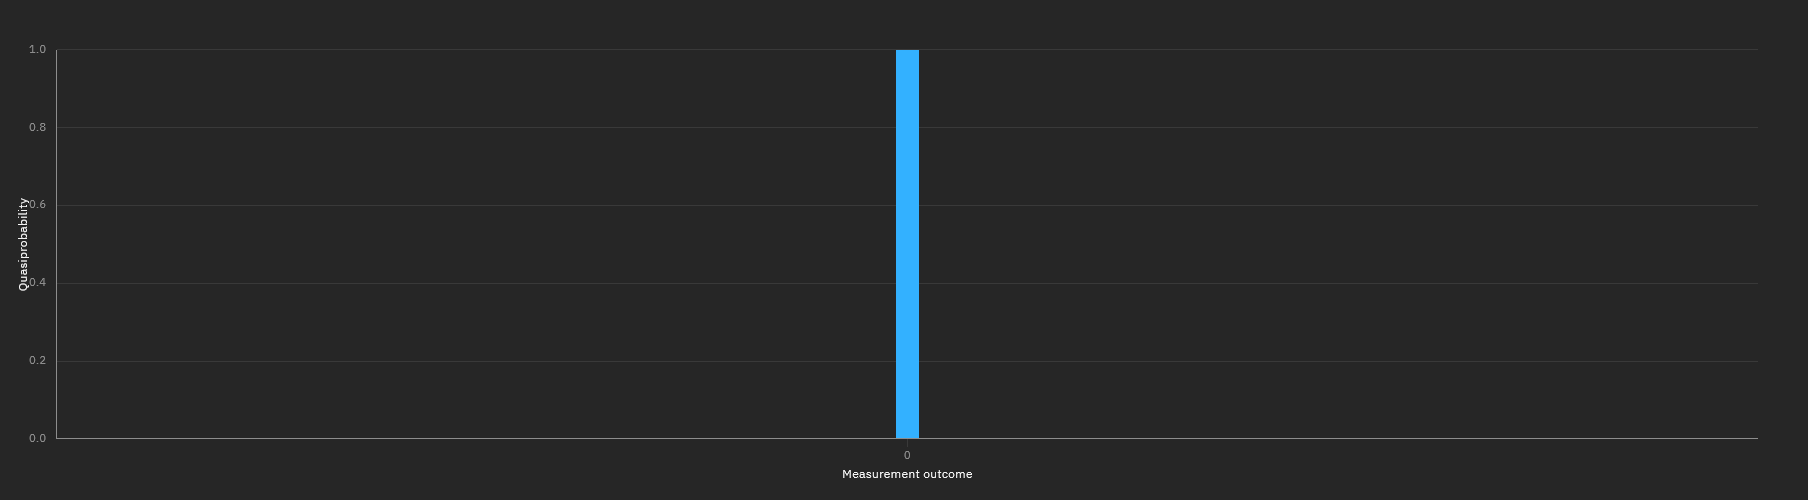
\includegraphics[scale=0.27]{1dr.png}
    \caption{The results of the measurement of the circuit after 1024 shots (on simulator).}
\end{figure}

\newpage

% part 2
\section*{Part 2}

% f(x) = x0 ⊕ x1 ⊕ x2 f : {0, 1}3 → {0, 1}
\subsection*{\text{a)}}

This is a balanced function and here is the implementation of the circuit and measurement outcome:

\begin{figure}[H]
    \centering
    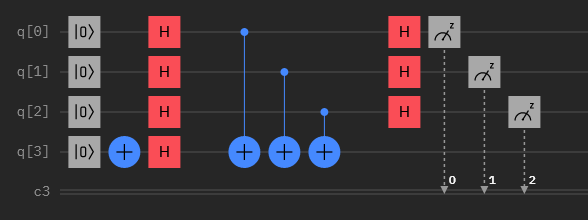
\includegraphics[scale=0.9]{2a.png}
    \caption{The circuit}
\end{figure}

\begin{figure}[H]
    \centering
    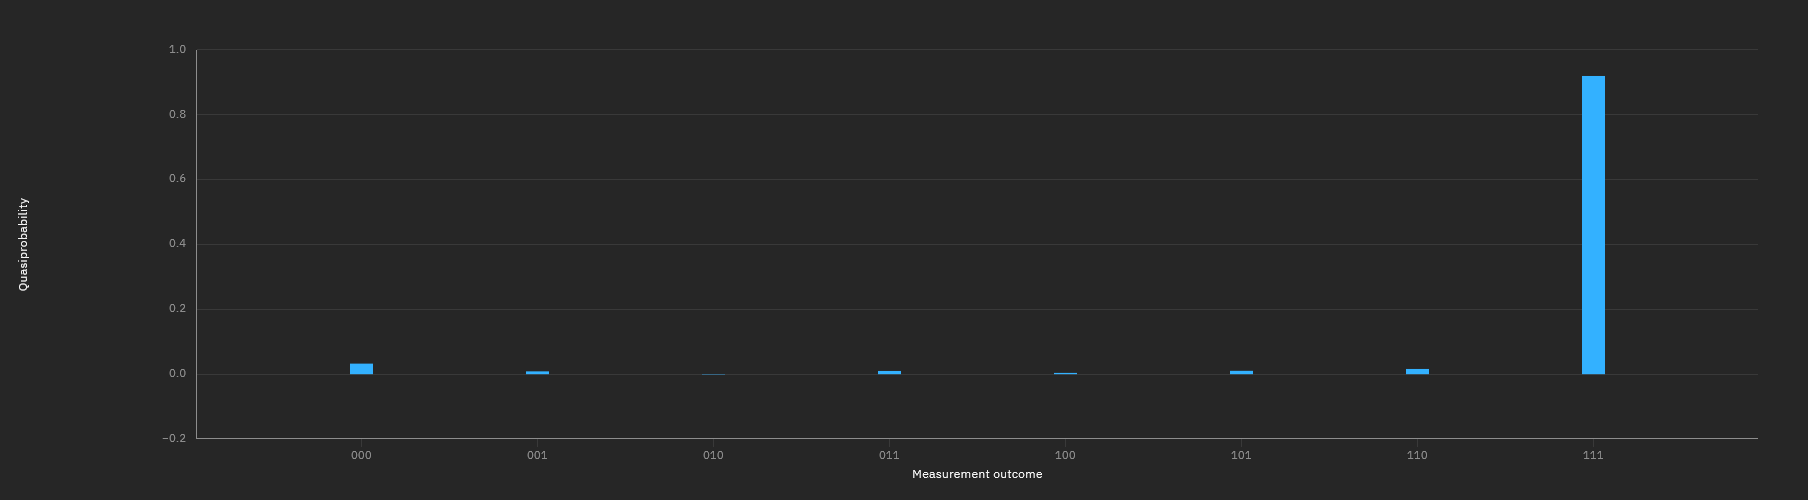
\includegraphics[scale=0.27]{2ar.png}
    \caption{The results of the measurement of the circuit after 1024 shots.}
\end{figure}

\newpage 

% f(x) = 1 and f : {0, 1}2 → {0, 1}
\subsection*{\text{b)}}

This is a constant function and here is the implementation of the circuit and measurement outcome:

\begin{figure}[H]
    \centering
    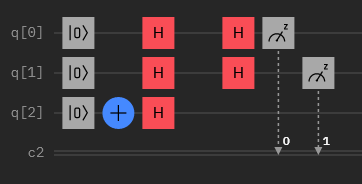
\includegraphics[scale=0.9]{2b.png}
    \caption{The circuit}
\end{figure}

\begin{figure}[H]
    \centering
    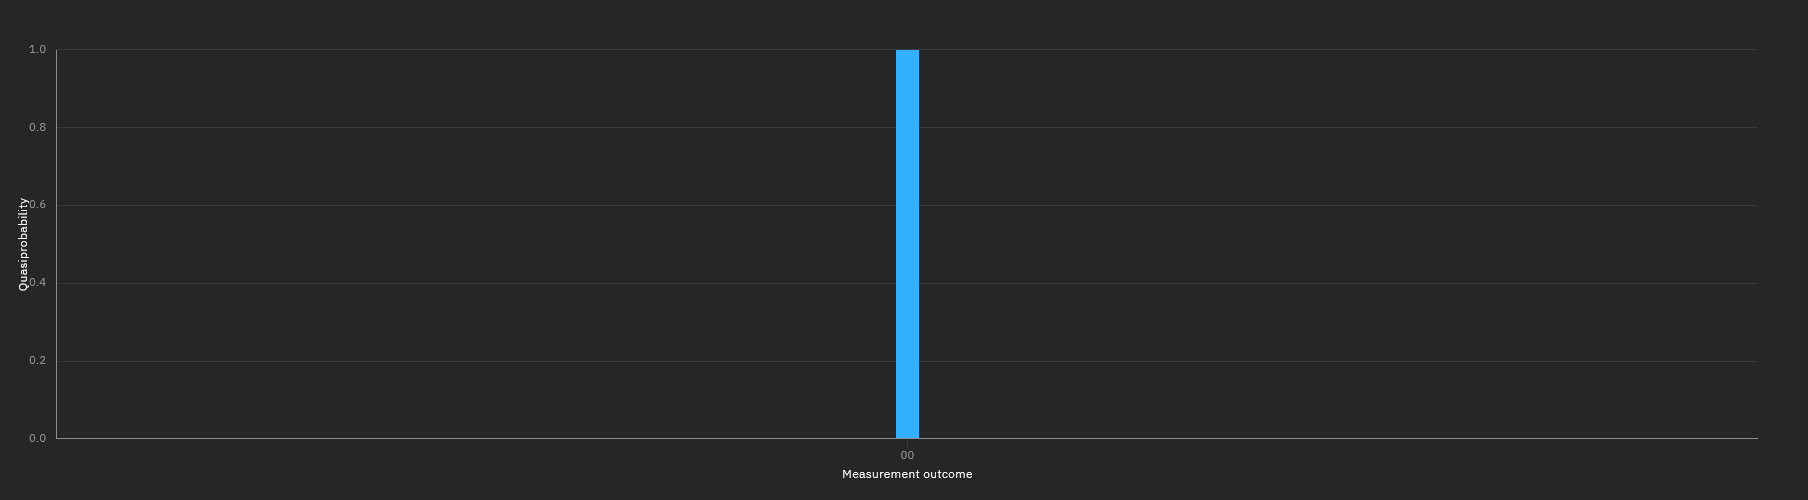
\includegraphics[scale=0.27]{2br.png}
    \caption{The results of the measurement of the circuit after 1024 shots (on simulator).}
\end{figure}

\newpage

% f(x) = x0 ⊕ x3 ⊕ (x1 · x2) and f : {0, 1}4 → {0, 1}
\subsection*{\text{c)}}

This is a balanced function and here is the implementation of the circuit and measurement outcome:

\begin{figure}[H]
    \centering
    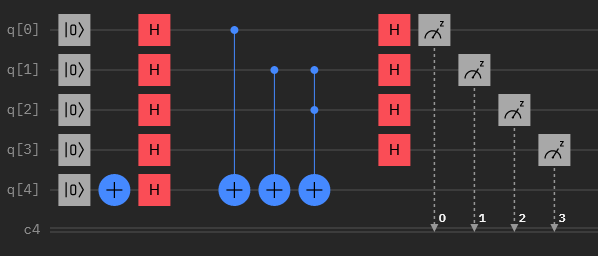
\includegraphics[scale=0.9]{2c.png}
    \caption{The circuit}
\end{figure}

\begin{figure}[H]
    \centering
    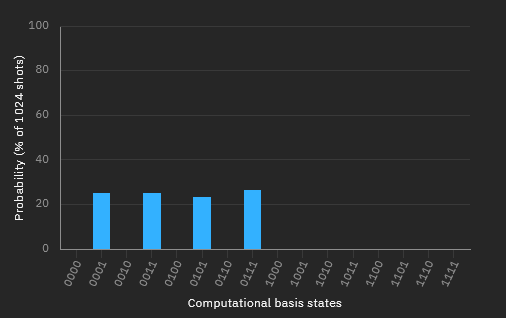
\includegraphics[scale=0.8]{2cr.png}
    \caption{The results of the measurement of the circuit after 1024 shots (on simulator).}
\end{figure}

\newpage

% the qiskit codes are here for each part separately
\section*{Appendix}

% 1 c
\subsection*{\text{1-c)}}

\begin{verbatim}
    from qiskit import QuantumRegister, ClassicalRegister, QuantumCircuit
    from numpy import pi

    qreg_q = QuantumRegister(2, 'q')
    creg_c = ClassicalRegister(1, 'c')
    circuit = QuantumCircuit(qreg_q, creg_c)

    circuit.reset(qreg_q[0])
    circuit.reset(qreg_q[1])
    circuit.x(qreg_q[1])
    circuit.h(qreg_q[0])
    circuit.h(qreg_q[1])
    circuit.cx(qreg_q[0], qreg_q[1])
    circuit.h(qreg_q[0])
    circuit.measure(qreg_q[0], creg_c[0])
    # @columns [0,0,1,2,2,3,4,5]

\end{verbatim}

% 1 d
\subsection*{\text{1-d)}}

\begin{verbatim}
    from qiskit import QuantumRegister, ClassicalRegister, QuantumCircuit
    from numpy import pi

    qreg_q = QuantumRegister(2, 'q')
    creg_c = ClassicalRegister(1, 'c')
    circuit = QuantumCircuit(qreg_q, creg_c)

    circuit.reset(qreg_q[0])
    circuit.reset(qreg_q[1])
    circuit.h(qreg_q[0])
    circuit.x(qreg_q[1])
    circuit.h(qreg_q[0])
    circuit.h(qreg_q[1])
    circuit.measure(qreg_q[0], creg_c[0])
    # @columns [0,0,1,1,2,2,3]
\end{verbatim}

\newpage

% 2 a
\subsection*{\text{2-a)}}

\begin{verbatim}
    from qiskit import QuantumRegister, ClassicalRegister, QuantumCircuit
    from numpy import pi
    
    qreg_q = QuantumRegister(4, 'q')
    creg_c = ClassicalRegister(3, 'c')
    circuit = QuantumCircuit(qreg_q, creg_c)
    
    circuit.reset(qreg_q[0])
    circuit.reset(qreg_q[1])
    circuit.reset(qreg_q[2])
    circuit.reset(qreg_q[3])
    circuit.x(qreg_q[3])
    circuit.h(qreg_q[0])
    circuit.h(qreg_q[1])
    circuit.h(qreg_q[2])
    circuit.h(qreg_q[3])
    circuit.CX(qreg_q[0], qreg_q[3])
    circuit.cx(qreg_q[1], qreg_q[3])
    circuit.cx(qreg_q[2], qreg_q[3])
    circuit.h(qreg_q[0])
    circuit.h(qreg_q[1])
    circuit.h(qreg_q[2])
    circuit.measure(qreg_q[0], creg_c[0])
    circuit.measure(qreg_q[1], creg_c[1])
    circuit.measure(qreg_q[2], creg_c[2])
    # @columns [0,0,0,0,1,2,2,2,2,4,5,6,8,8,8,9,10,11]
\end{verbatim}

% 2 b
\subsection*{\text{2-b)}}

\begin{verbatim}
    from qiskit import QuantumRegister, ClassicalRegister, QuantumCircuit
    from numpy import pi
    
    qreg_q = QuantumRegister(3, 'q')
    creg_c = ClassicalRegister(2, 'c')
    circuit = QuantumCircuit(qreg_q, creg_c)
    
    circuit.reset(qreg_q[0])
    circuit.reset(qreg_q[1])
    circuit.reset(qreg_q[2])
    circuit.x(qreg_q[2])
    circuit.h(qreg_q[0])
    circuit.h(qreg_q[1])
    circuit.h(qreg_q[2])
    circuit.h(qreg_q[0])
    circuit.h(qreg_q[1])
    circuit.measure(qreg_q[0], creg_c[0])
    circuit.measure(qreg_q[1], creg_c[1])
    # @columns [0,0,0,1,2,2,2,4,4,5,6]
\end{verbatim}

% 2 c
\subsection*{\text{2-c)}}

\begin{verbatim}
    from qiskit import QuantumRegister, ClassicalRegister, QuantumCircuit
    from numpy import pi

    qreg_q = QuantumRegister(5, 'q')
    creg_c = ClassicalRegister(4, 'c')
    circuit = QuantumCircuit(qreg_q, creg_c)

    circuit.reset(qreg_q[0])
    circuit.reset(qreg_q[1])
    circuit.reset(qreg_q[2])
    circuit.reset(qreg_q[3])
    circuit.reset(qreg_q[4])
    circuit.x(qreg_q[4])
    circuit.h(qreg_q[0])
    circuit.h(qreg_q[1])
    circuit.h(qreg_q[2])
    circuit.h(qreg_q[3])
    circuit.h(qreg_q[4])
    circuit.cx(qreg_q[0], qreg_q[4])
    circuit.cx(qreg_q[1], qreg_q[4])
    circuit.ccx(qreg_q[1], qreg_q[2], qreg_q[4])
    circuit.h(qreg_q[0])
    circuit.h(qreg_q[1])
    circuit.h(qreg_q[2])
    circuit.h(qreg_q[3])
    circuit.measure(qreg_q[0], creg_c[0])
    circuit.measure(qreg_q[1], creg_c[1])
    circuit.measure(qreg_q[2], creg_c[2])
    circuit.measure(qreg_q[3], creg_c[3])
    # @columns [0,0,0,0,0,1,2,2,2,2,2,4,5,6,8,8,8,8,9,10,11,12]
\end{verbatim}


\end{document}
